\documentclass[10pt]{beamer}
\usetheme{Madrid}
\usepackage{booktabs}
\usepackage{graphicx}
\usepackage[T1]{fontenc}
\usepackage{tikz}
\usetikzlibrary{arrows.meta}
\setbeamertemplate{navigation symbols}{}
% To view speaker notes, uncomment the next line (adds note pages):
% \setbeameroption{show notes}
\tikzset{
  box/.style={draw, rounded corners, align=center, text width=2.3cm, minimum height=0.9cm, font=\scriptsize},
  kuser/.style={box, fill=blue!15}, kagent/.style={box, fill=green!25},
  kdata/.style={box, fill=black!8}, kdanger/.style={box, fill=red!25},
  koutput/.style={box, fill=orange!25}, kdecision/.style={box, fill=yellow!30},
  kguard/.style={box, fill=violet!25},
  flow/.style={-{Stealth[length=2mm]}, thick},
}
% ======================= EDIT YOUR DETAILS =======================
\newcommand{\studentname}{Aflah Muhammed P}
% Change the university roll/registration number:
\newcommand{\rollno}{TVE23CSXXX}
% Change your class roll number:
\newcommand{\rollclass}{Roll No: XX}
% Change your guide name:
\newcommand{\guidename}{Prof. Guide Name}
% Change department / college / short-institute if needed:
\newcommand{\deptname}{Department of Computer Science and Engineering}
\newcommand{\collegename}{College of Engineering Trivandrum}
\newcommand{\shortinst}{CET}
% Change the seminar date:
\newcommand{\seminardate}{\today}
% =================================================================
\title[B.Tech Seminar]{Orchestrating Teams of AI Agents: Architecture, Protocols, and Real-World Adoption}
\subtitle{Based on: The Orchestration of Multi-Agent Systems: Architectures, Protocols, and Enterprise Adoption (arXiv:2601.13671, 2026)}
\author[\studentname\ (\shortinst)]{\studentname \\ \small \rollno \\ \small \rollclass \\ \small Guide: \guidename}
\institute[]{\deptname \\ \collegename}
\date{\seminardate}
\begin{document}
\begin{frame}[plain]
  \titlepage
\end{frame}
\begin{frame}{Table of Contents}
  \tableofcontents
\end{frame}
\section{Introduction}
\begin{frame}{Introduction}
\begin{itemize}
  \item An AI agent is a program that uses a language model to decide and act.
  \item One agent often struggles with big, multi-step, real-world tasks.
  \item Multi-agent systems split the work across specialized, cooperating agents.
  \item An orchestration layer coordinates those agents like a project manager.
  \item Two open standards, MCP and A2A, let agents talk safely.
  \item This paper unifies the architecture, the protocols, and enterprise adoption advice.
\end{itemize}
\end{frame}
\note{Let's start simple. An AI agent is just a program that uses a language model to think and act on its own. One agent is fine for small jobs, but big real-world tasks need several agents working together, coordinated by an orchestration layer. Today we'll see how this paper organizes that teamwork and lets the agents talk through two open standards, MCP and A2A.}
\section{Literature Survey}
\begin{frame}{Literature Survey / Background}
  \small
  \begin{tabular}{@{}p{2.7cm}p{2.3cm}p{5.6cm}@{}}
    \toprule
    \textbf{Title} & \textbf{Author} & \textbf{Summary} \\
    \midrule
    AutoGen: Multi-Agent Conversation Framework & Wu et al. (2023) & Framework where multiple LLM agents converse to solve tasks, an early model for agent collaboration this paper generalizes. \\
    \addlinespace
    ReAct: Reasoning and Acting in Language Models & Yao et al. (2023) & Shows a single agent interleaving reasoning steps with tool actions, the loop that orchestration scales to many agents. \\
    \addlinespace
    Model Context Protocol Specification & Anthropic (2024) & Open standard for connecting agents to external tools and data, one of the two protocols this paper formalizes. \\
    \addlinespace
    \bottomrule
  \end{tabular}
\end{frame}
\note{This idea didn't appear from nowhere. AutoGen showed agents can solve problems by talking to each other, and ReAct showed a single agent interleaving reasoning with tool use. The Model Context Protocol then standardized how agents reach tools. This paper builds on all three and pulls them into one coherent enterprise framework.}
\section{Motivation}
\begin{frame}{Motivation}
\begin{itemize}
  \item Single agents lose context and skip steps during long, complex tasks.
  \item Enterprises need reliable, auditable AI, not just impressive one-off demos.
  \item Hand-written glue code between agents and tools rarely scales or lasts.
  \item Without shared standards, agents from different vendors cannot cooperate.
  \item Businesses want measurable productivity gains alongside governance and safety.
\end{itemize}
\end{frame}
\note{Why bother with many agents? Because a single agent tends to forget context and drop steps in long tasks. Companies also need systems they can audit and trust, not just flashy demos. And when every team hand-codes its own connections, nothing scales, so shared standards really matter.}
\section{Problem Statement}
\begin{frame}{Problem Statement}
  \begin{block}{}
  Building dependable systems of many cooperating AI agents is hard because coordination, tool access, shared state, and safety are usually improvised per project. The paper asks how to unify these into one architecture with standard, auditable communication fit for enterprises.
  \end{block}
\end{frame}
\note{Here is the core problem. Coordinating many agents, giving them tool access, keeping shared memory, and staying safe are usually improvised for each project. The paper asks how to combine all of that into one architecture with communication that is standardized and auditable enough for real businesses.}
\section{Objectives}
\begin{frame}{Objectives}
\begin{itemize}
  \item Define a unified architecture for orchestrating many cooperating agents.
  \item Explain planning, policy, state, and quality control as core layers.
  \item Detail MCP for standardized agent-to-tool and data access.
  \item Detail A2A for agent-to-agent coordination, negotiation, and delegation.
  \item Provide governance and observability practices for trust and auditability.
  \item Give enterprises a practical, phased path to safe adoption.
\end{itemize}
\end{frame}
\note{So the goals are clear. Define one architecture for many cooperating agents, and explain its core pieces: planning, policy, state, and quality control. Then detail the two protocols, MCP for tools and A2A for agent-to-agent talk. Finally, add governance and give enterprises a safe, step-by-step adoption path.}
\section{Methodology}
\begin{frame}[allowframebreaks]{Methodology: The Orchestration Layer}
\begin{itemize}
  \item Planning breaks one big goal into ordered sub-tasks.
  \item Policy enforcement checks every proposed action against rules.
  \item State management keeps shared memory consistent across agents.
  \item Quality operations validate outputs and trigger retries when needed.
  \item It acts as the manager translating goals into agent work.
\end{itemize}
\end{frame}
\note{Think of the orchestration layer as a project manager. It plans the work, enforces the rules, keeps shared memory consistent, and checks quality. The two protocols are how the team communicates: MCP is how an agent picks up a tool, and A2A is how agents hand work to each other. Wrapped around everything is governance that logs and limits what agents can do.}
\begin{frame}[allowframebreaks]{Methodology: Communication Protocols: MCP and A2A}
\begin{itemize}
  \item MCP is a client-server standard for calling tools and data.
  \item MCP lets any agent use any MCP-compatible tool safely.
  \item A2A carries structured messages so agents delegate and negotiate.
  \item A2A adds acknowledgments and retries for reliable handoffs.
  \item Together they form one interoperable communication substrate.
\end{itemize}
\end{frame}
\begin{frame}[allowframebreaks]{Methodology: Governance and Observability}
\begin{itemize}
  \item Access controls whitelist which tools each agent may use.
  \item Audit trails log every decision for later review.
  \item Tracing and metrics track latency, cost, and error rates.
  \item Human approval gates guard high-stakes or irreversible actions.
\end{itemize}
\end{frame}
\section{Key Concepts}
\begin{frame}[allowframebreaks]{Key Concepts}
  \begin{description}
    \item[AI Agent] Software that uses a language model to reason and take actions toward a goal.
    \item[Orchestration Layer] The coordinator that plans, assigns, and supervises agents like a manager.
    \item[MCP (Model Context Protocol)] Open standard letting agents call external tools and data in a uniform way.
    \item[A2A (Agent2Agent)] Open standard letting agents message, delegate, and negotiate with each other.
    \item[Shared State] Common memory so agents stay consistent across task handoffs.
    \item[Governance] Policies, access limits, and audit logs keeping the system safe and accountable.
  \end{description}
\end{frame}
\note{Let's lock in the vocabulary. An agent reasons and acts toward a goal. The orchestration layer is the manager coordinating agents. MCP is the standard plug for tools and data, while A2A is the standard for agents talking to each other. Shared state is the common memory, and governance is the rules and logs that keep it all safe.}
\section{System Architecture}
\begin{frame}{System Architecture}
  \begin{center}
  \resizebox{0.96\textwidth}{!}{%
  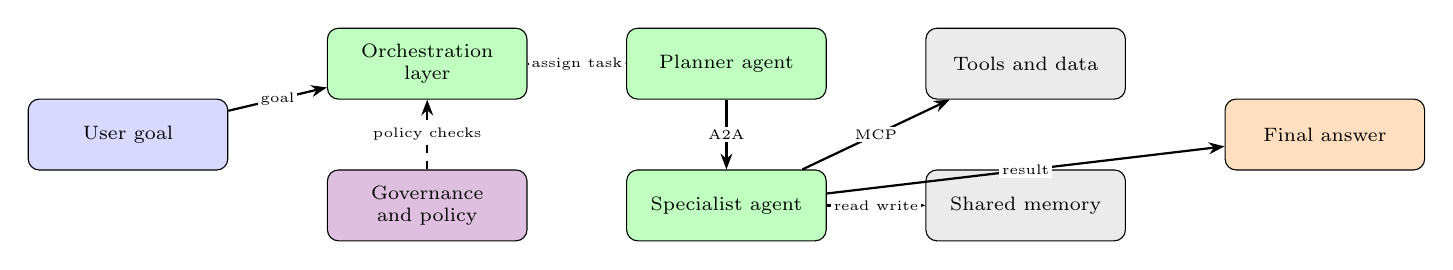
\begin{tikzpicture}
    \node[kuser] (user) at (0.00,0.00) {User goal};
    \node[kagent] (orch) at (3.80,0.90) {Orchestration layer};
    \node[kguard] (gov) at (3.80,-0.90) {Governance and policy};
    \node[kagent] (planner) at (7.60,0.90) {Planner agent};
    \node[kagent] (worker) at (7.60,-0.90) {Specialist agent};
    \node[kdata] (tools) at (11.40,0.90) {Tools and data};
    \node[kdata] (state) at (11.40,-0.90) {Shared memory};
    \node[koutput] (output) at (15.20,0.00) {Final answer};
    \draw[flow] (user) -- (orch) node[midway, font=\tiny, fill=white, inner sep=1pt]{goal};
    \draw[flow] (orch) -- (planner) node[midway, font=\tiny, fill=white, inner sep=1pt]{assign task};
    \draw[flow] (planner) -- (worker) node[midway, font=\tiny, fill=white, inner sep=1pt]{A2A};
    \draw[flow] (worker) -- (tools) node[midway, font=\tiny, fill=white, inner sep=1pt]{MCP};
    \draw[flow, dashed] (worker) -- (state) node[midway, font=\tiny, fill=white, inner sep=1pt]{read write};
    \draw[flow, dashed] (gov) -- (orch) node[midway, font=\tiny, fill=white, inner sep=1pt]{policy checks};
    \draw[flow] (worker) -- (output) node[midway, font=\tiny, fill=white, inner sep=1pt]{result};
  \end{tikzpicture}%
  }
  \end{center}
  \begin{center}\scriptsize How the orchestration layer routes a user goal through governed agents that use A2A and MCP to produce a final answer.\end{center}
\end{frame}
\note{Follow the diagram left to right. The user's goal enters the orchestration layer, which plans the work while a governance guard checks and logs every action. The orchestrator hands tasks to specialist agents that cooperate over A2A. Those agents reach tools and data through MCP and share memory, then their validated results become the final answer on the right.}
\begin{frame}[allowframebreaks]{How It Works (Explained)}
\begin{itemize}
  \item A user submits a goal on the far left of the diagram.
  \item The orchestration layer receives it and plans the sub-tasks.
  \item A governance and policy guard wraps the orchestrator, checking and logging actions.
  \item The orchestrator assigns work to specialist agents that cooperate over A2A.
  \item Agents reach external tools and data through MCP, and read or write shared memory.
  \item Validated results are aggregated into the final answer on the right.
\end{itemize}
\end{frame}
\section{Example Walkthrough}
\begin{frame}[allowframebreaks]{Example Walkthrough: Example: Reviewing an insurance contract for risky clauses}
\begin{enumerate}
  \item A user uploads a contract PDF and asks the system to flag risky clauses.
  \item The orchestrator plans: extract text, analyze clauses, then summarize risks.
  \item It assigns a planner agent, which delegates to a specialist over A2A.
  \item The specialist uses MCP to open the PDF tool and a legal-clause database.
  \item Governance confirms the agent may read that data and logs the access.
  \item Agents write findings to shared state and quality-check them for errors.
  \item The orchestrator aggregates a plain-language risk summary and returns it to the user.
\end{enumerate}
\end{frame}
\note{Let's make it concrete with a contract review. A user uploads a PDF and asks which clauses are risky. The orchestrator plans the steps, delegates to a specialist over A2A, and that agent uses MCP to open the document and a legal database. Governance approves and logs the access, the agents verify their findings, and the orchestrator returns a plain-language risk summary.}
\section{Results}
\begin{frame}[allowframebreaks]{Results / Findings}
\begin{itemize}
  \item The paper is a synthesis and framework; its evidence comes from cited industry studies, not one benchmark.
  \item McKinsey estimates agentic AI can lift knowledge-work productivity by roughly 15-30 percent.
  \item Reported document-processing and support use cases show about 30-40 percent efficiency gains.
  \item Cited deployments report 30-60 percent faster resolution than manual processes.
  \item Standardized protocols are estimated to cut integration effort by around 25-35 percent.
  \item Production agents in cited cases report task success rates near 85-95 percent.
\end{itemize}
\end{frame}
\note{A quick honesty note first: this is a framework paper, so its numbers come from cited industry studies, not one experiment. With that caveat, McKinsey estimates 15 to 30 percent productivity gains, document and support tasks show 30 to 40 percent efficiency improvements, and standard protocols cut integration effort by roughly a quarter to a third. Treat these as encouraging directional evidence, not guarantees.}
\section{Discussion}
\begin{frame}{Discussion}
\begin{itemize}
  \item The layered design separates concerns, so planning, safety, and tools evolve independently.
  \item Shared open protocols reduce vendor lock-in and let mixed agent fleets cooperate.
  \item Governance and observability are treated as first-class, not afterthoughts, which suits regulated industries.
  \item The reported gains are promising but come mostly from early adopters and vendor studies.
\end{itemize}
\end{frame}
\note{What makes this design attractive is separation of concerns: planning, safety, and tools can each improve on their own. Open protocols reduce vendor lock-in so mixed agent fleets can cooperate. And because governance and observability are built in, the approach fits regulated industries, though the reported gains still lean on early adopters.}
\section{Challenges}
\begin{frame}{Limitations \& Challenges}
\begin{itemize}
  \item The paper is largely conceptual, with limited original controlled experiments.
  \item Quoted numbers are industry-cited ranges that vary widely by task and setting.
  \item MCP and A2A are young standards still evolving toward broad adoption.
  \item More agents add coordination overhead, latency, and new security surfaces.
\end{itemize}
\end{frame}
\note{Let's be balanced. The paper is mostly conceptual with limited controlled experiments, and its numbers are wide industry ranges that depend heavily on the task. Both protocols are young and still evolving. And adding more agents brings coordination overhead, extra latency, and new security risks.}
\section{Future Work}
\begin{frame}{Future Work}
\begin{itemize}
  \item Run standardized benchmarks to measure orchestration cost and reliability directly.
  \item Harden protocols against prompt injection and malicious or faulty agents.
  \item Develop richer negotiation and planning strategies for larger agent teams.
  \item Publish reusable reference implementations and enterprise deployment blueprints.
\end{itemize}
\end{frame}
\note{Looking ahead, the field needs shared benchmarks to measure orchestration cost and reliability directly. Protocols should be hardened against prompt injection and misbehaving agents. Better planning and negotiation strategies will help larger teams, and open reference implementations would speed safe adoption.}
\section{Conclusion}
\begin{frame}{Conclusion}
\begin{itemize}
  \item Orchestrated multi-agent systems are a practical next step beyond single agents.
  \item A clear layer plus MCP and A2A gives a scalable, standard-based blueprint.
  \item Governance and observability make these systems trustworthy enough for enterprises.
  \item Beginners should focus on the pattern: plan, delegate, use tools, verify, govern.
\end{itemize}
\end{frame}
\note{To wrap up, orchestrated multi-agent systems are a sensible next step beyond a single agent. A clear orchestration layer plus MCP and A2A gives a scalable, standards-based blueprint, and built-in governance makes it trustworthy enough for enterprises. If you remember one thing, remember the pattern: plan, delegate, use tools, verify, and govern.}
\section{References}
\begin{frame}[allowframebreaks]{References}
  \footnotesize
  \begin{enumerate}
    \item Adimulam, A., Gupta, R., \& Kumar, S. (2026). The Orchestration of Multi-Agent Systems: Architectures, Protocols, and Enterprise Adoption. arXiv:2601.13671. https://arxiv.org/abs/2601.13671
    \item Anthropic. (2024). Model Context Protocol (MCP) Specification. https://modelcontextprotocol.io
    \item Google. (2025). Agent2Agent (A2A) Protocol Announcement and Specification. https://a2aproject.github.io
    \item Wu, Q., et al. (2023). AutoGen: Enabling Next-Gen LLM Applications via Multi-Agent Conversation. arXiv:2308.08155.
    \item Yao, S., et al. (2023). ReAct: Synergizing Reasoning and Acting in Language Models. arXiv:2210.03629.
    \item McKinsey \& Company. (2025). The Agentic AI Advantage: Superagency in the Workplace.
  \end{enumerate}
\end{frame}
\begin{frame}[plain]
  \begin{center}
    {\Huge Thank You}\\[1em]
    {\large Questions?}
  \end{center}
\end{frame}
\end{document}